\section{Introduction and motivation}
\label{sec:Introduction}

%This is the reference~\cite{Gligorov:2017nwh}
%\newline
%\textbf{``The results shown are unofficial and have not been formally approved by the LHCb collaboration"}

%\subsection{Motivations}

The discovery of the Higgs at the LHC in 2012 filled in the last missing piece of the Standard Model (SM). Apart from a few so-called ``anomalies'', mostly in the flavor sector, the SM has been a spectacular successly theoretical framework that can account for all observed phenomena. Yet, we know that it is also an incomplete theory that can not account for gravity, dark matter, observed matter-antimatter asymmetry in the universe, among other problems. NP searches at the LHC experiments have mostly focused on production of new particles that decay promptly, within the detector volume. However, an important NP portal is one that is very weakly coupled sector with the SM and therefore includes particles with long lifetimes. In fact, long lifetimes are very generic in any theory with multiple mass scales, broken symmetries, or restricted phase-space. The SM itself contains templates for low mass long lived particles (LLP) such as electron, neutrino, proton and neutron.
There are several experiments for searching longlived particles (LLPs). 
Likewise we introduce a new detector to measure LLPs based on high luminosity large hadron collider (HL-LHC).
%MATHUSLA (\atlas), MilliQan (\cms), SHiP. 
%But these experiments are so large to compare with CODEX-b, this is a one attractive of CODEX-b. 
%We can control backgrounds because it will be placed underground and shields are existed. 

\begin{figure}
\centering
    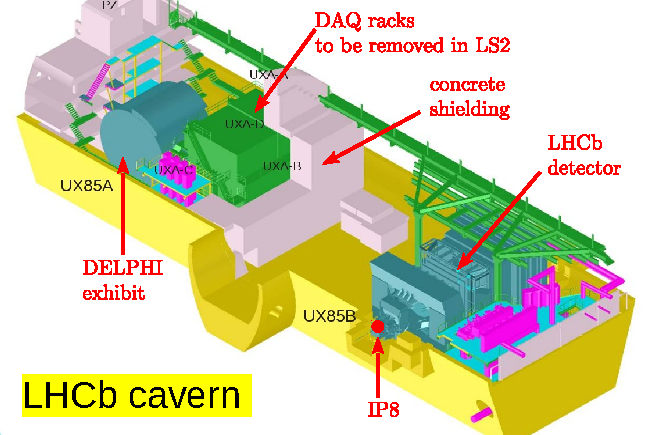
\includegraphics[width=15cm]{figs/INT/lhcb_cavern.pdf}
\caption{ 
   A schematic plot of the LHCb cavern. 
}
\end{figure}


\subsection{Compact Detector for Exotics at LHCb}

The Compact Detector for Exotics at \lhcb (CODEX-b) was proposed to detect weakly coupled LLPs in \lhcb cavern. 
Since \atlas and \cms focused on high \pt and large QCD backgrounds and restricted lifetime of \lhcb, current detectors can miss signals from weakly coupled LLPs. 
By following the fig.~1, the DAQ racks will be moved to the surface before run~3 and the CODEX-b will be placed at the site with 10 X 10 X 10~m size. 
The CODEX-b aparts 25~m from the impact point~8. 
If the \delphi is removed, the size can be expanded to 20 X 10 X 10~m.
%The CODEX-b consists of two parts. 
%6 RPC layers at 4\cm intervals on each box face with 1\cm granularity (Attach the geometry plot of CODEX-b here!!). 
%5 equally spaced triplets along the depth to minimize distance between reconstructed vertex and 1st measurement. 
%50 - 100 ps timing from RPC's foreseenfor mass reconstruction.
%Additional passive Pb shield to suppress muon and neutral hadrons. 
%Thin active veto for secondaries inside the shield. 


\subsection{Other detector proposals for searching LLPs at LHC}

Not only the CODEX-b but also there are other detector proposals to search long-lived particles at LHC.
The MATHUSLA (MAssive Timing Hodoscope for Ultra Stable neutraL pArticles), the milliQan and the FASER (ForwArd Search ExpeRiment at the LHC) are based on the collider experiment. 
Also, there is a detector based on beam dump experiment called the SHiP (Search for Hidden Particles).
CODEX-b has advantages comparing other detectors.
Since the CODEX-b will be implemented underground and next to the concrete wall, it is easy to control background.
It is expected that cosmic rays are blocked by ground and particles from beam collisions are blocked by the concrete wall.
Also it will take less price because it plans to use existed place and equipments.

